% chapter07.tex

 %%%%%%%%%%%%%%%%%%%%%%%%%%%%%%%%%%%%%%%%%%%%%%%%%%%%%%%%%%%%%%%%%%%%%%%%%%%%%
 %                                                                           %
 %    PyMS documentation                                                     %
 %    Copyright (C) 2005-8 Vladimir Likic                                    %
 %                                                                           %
 %    The files in this directory provided under the Creative Commons        %
 %    Attribution-NonCommercial-NoDerivs 2.1 Australia license               %
 %    http://creativecommons.org/licenses/by-nc-nd/2.1/au/                   %
 %    See the file license.txt                                               %
 %                                                                           %
 %%%%%%%%%%%%%%%%%%%%%%%%%%%%%%%%%%%%%%%%%%%%%%%%%%%%%%%%%%%%%%%%%%%%%%%%%%%%%

\chapter{Displaying information using the Display Module}

PyMS can be used to display information such as Ion Chromatograms (ICs), 
Total Ion Chromatogram (TIC) and detected lists of peaks. This functionality
is provided by the package matplotlib, which must be installed in order 
to use the Display module and to run the scripts referred to in this chapter



\section{Displaying the Total Ion Chromatogram (TIC) of a data object}
\label{sec:DisplayTic}
\noindent
[ {\em This example is in pyms-test/70a} ]

To display the TIC, it must first be extracted from the data. This is done as 
in section \ref{sec:IonChromatogramObject}. Having found
and stored the TIC object, a simple call to the function {\tt plot\_ics()} displays
the TIC in a new window. In addition to the TIC, two strings may be passed to plot\_ics()
which label the data (in this case 'TIC'), and the overall plot ('TIC for gc01\_0812\_066').

\begin{verbatim}
>>> plot_ics(tic, 'TIC','TIC for gc01_0812_066')
\end{verbatim}

The following window should now be displayed:

\begin{center}
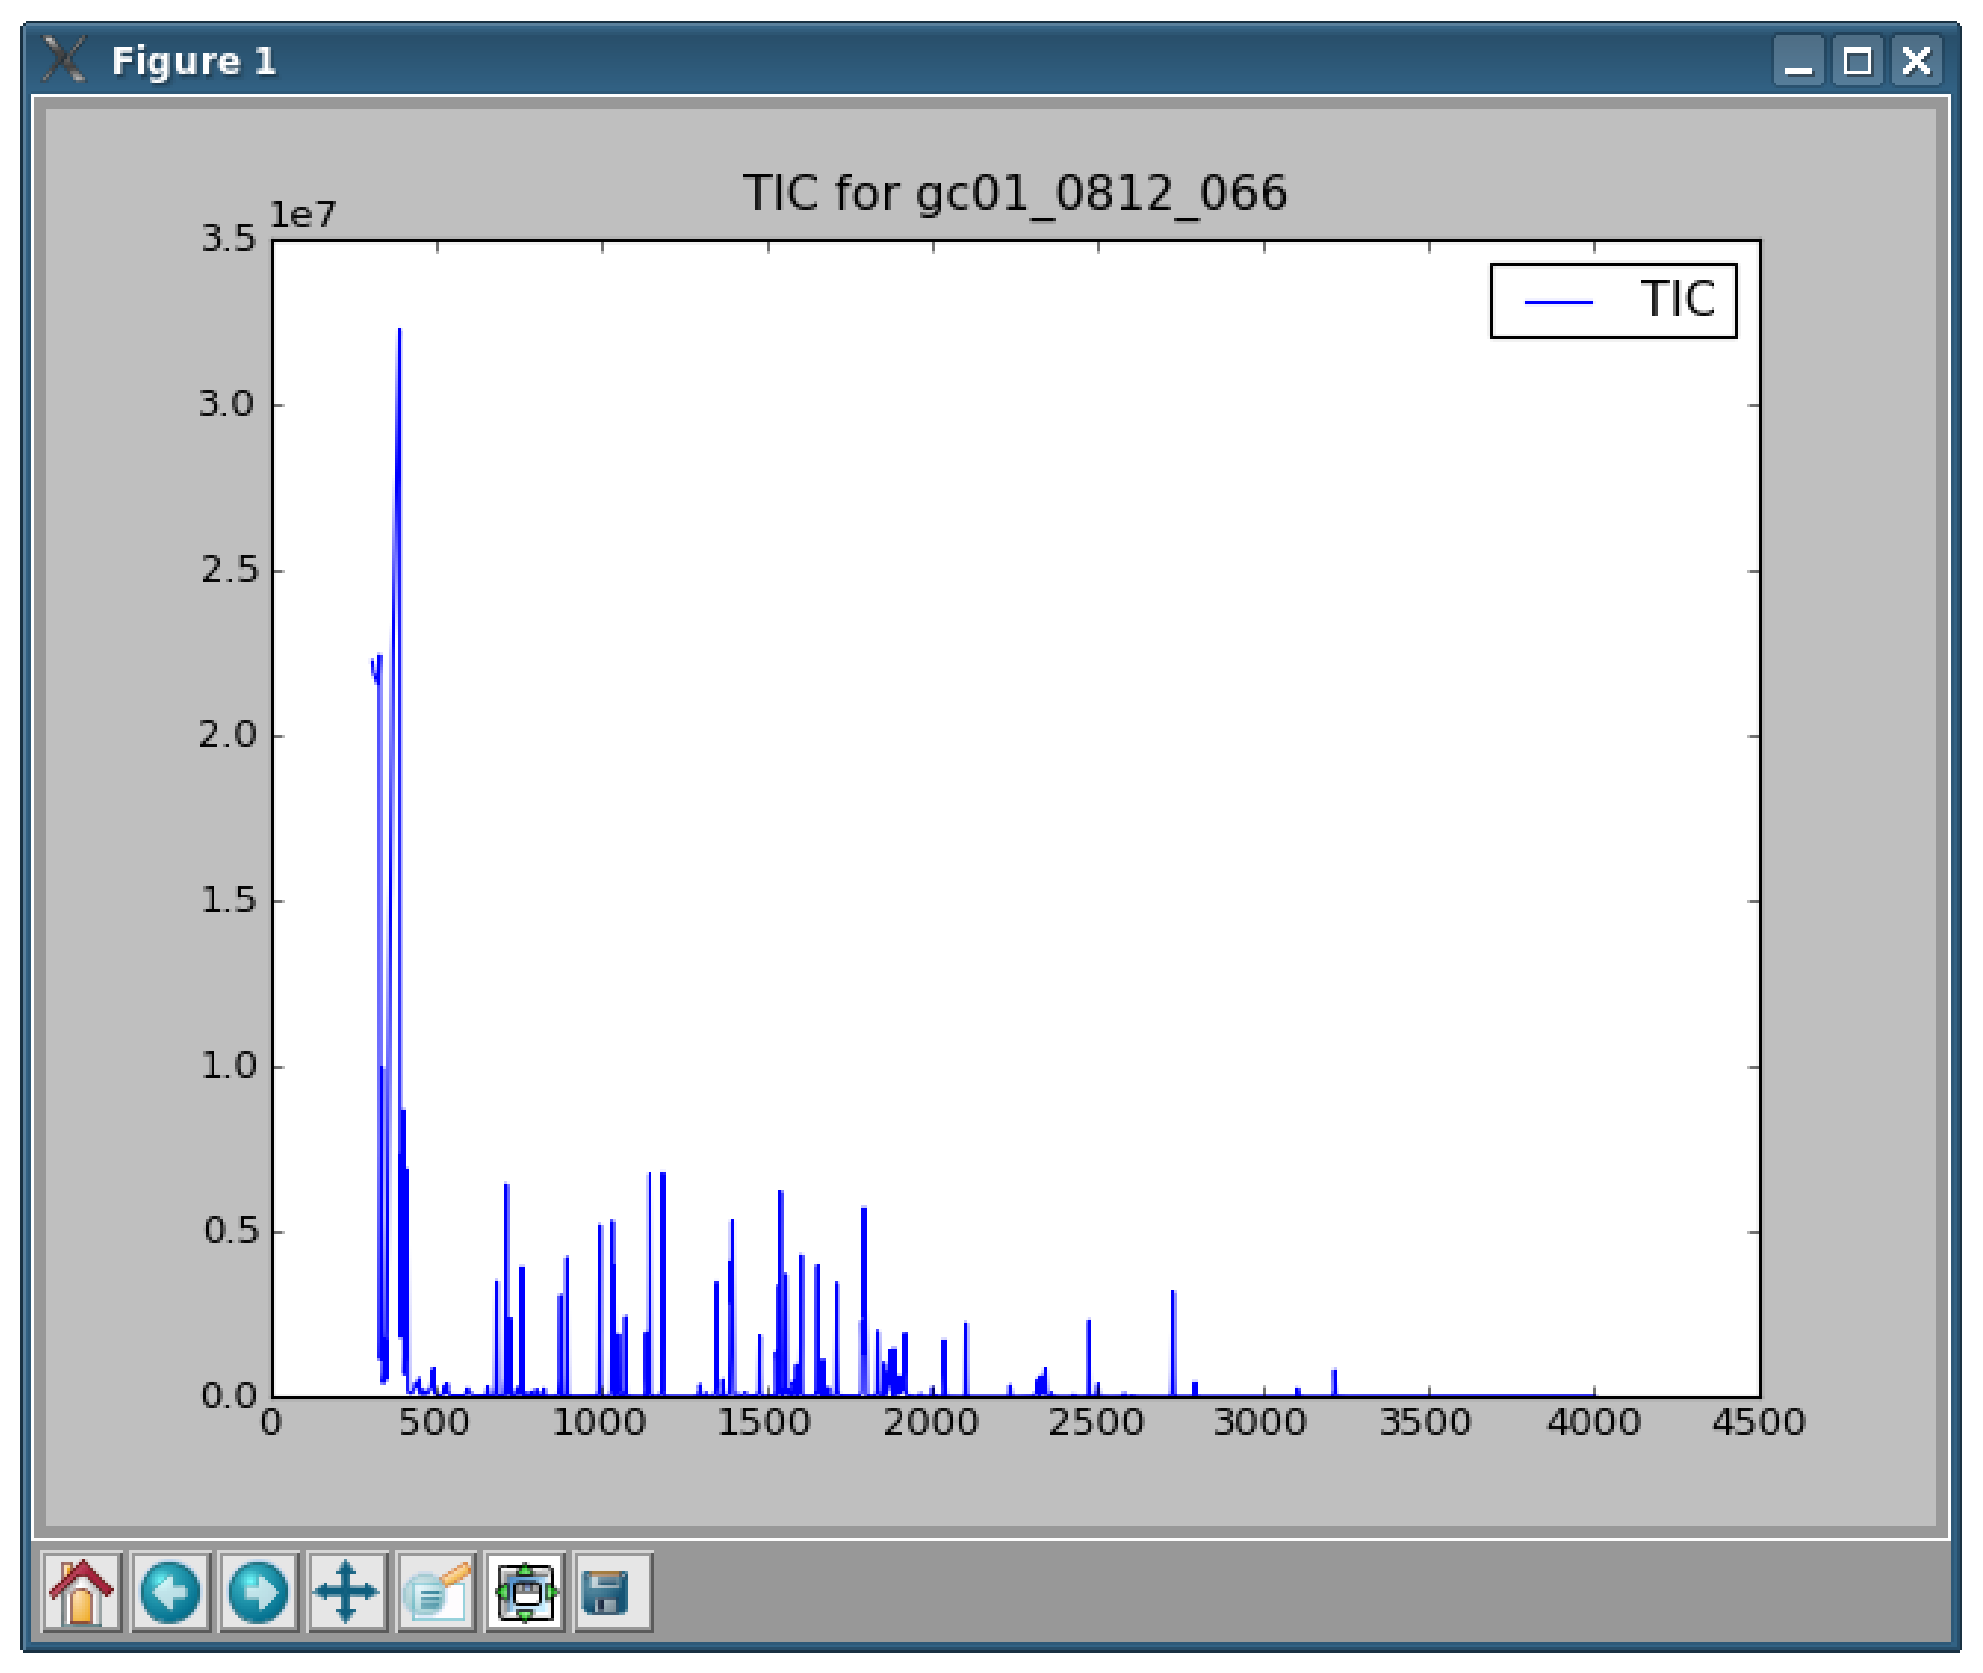
\includegraphics[scale=0.33]{graphics/chapter07/test-70a.eps}
\end{center}

To zoom in on a portion of the plot, select the

\includegraphics[scale=0.5]{graphics/chapter07/magnifier_button.eps}
button, then hold down the 
left mouse button while dragging a rectangle over the area of interest. To return
to the original view, simply click on the

\includegraphics[scale=0.5]{graphics/chapter07/home_button.eps}
button.

The 

\includegraphics[scale=0.5]{graphics/chapter07/cross_button.eps}
button allows panning across the zoomed plot. 


\section{Displaying multiple Ion Chromatograms and the TIC}

\noindent
[ {\em This example is in pyms-test/70b} ]


The Display module can plot multiple ICs and the TIC on the same figure, 
To do this, a list of Ion Chromatogram objects is created:

\begin{verbatim}
>>> tic = data.get_tic()
>>> ic = im.get_ic_at_mass(73)
>>> ic1 = im.get_ic_at_mass(147)
>>> ics = [tic, ic, ic1]
\end{verbatim}

This list is passed to the 
function {\tt plot\_ics()}, along with a list of strings to label each 
Ion Chromatogram:

\begin{verbatim}
>>> plot_ics(ics, ['TIC', '73','147'], 'TIC and ICs for m/z = 73 & 147')
\end{verbatim}

This should result in the following window being displayed:

\begin{center}
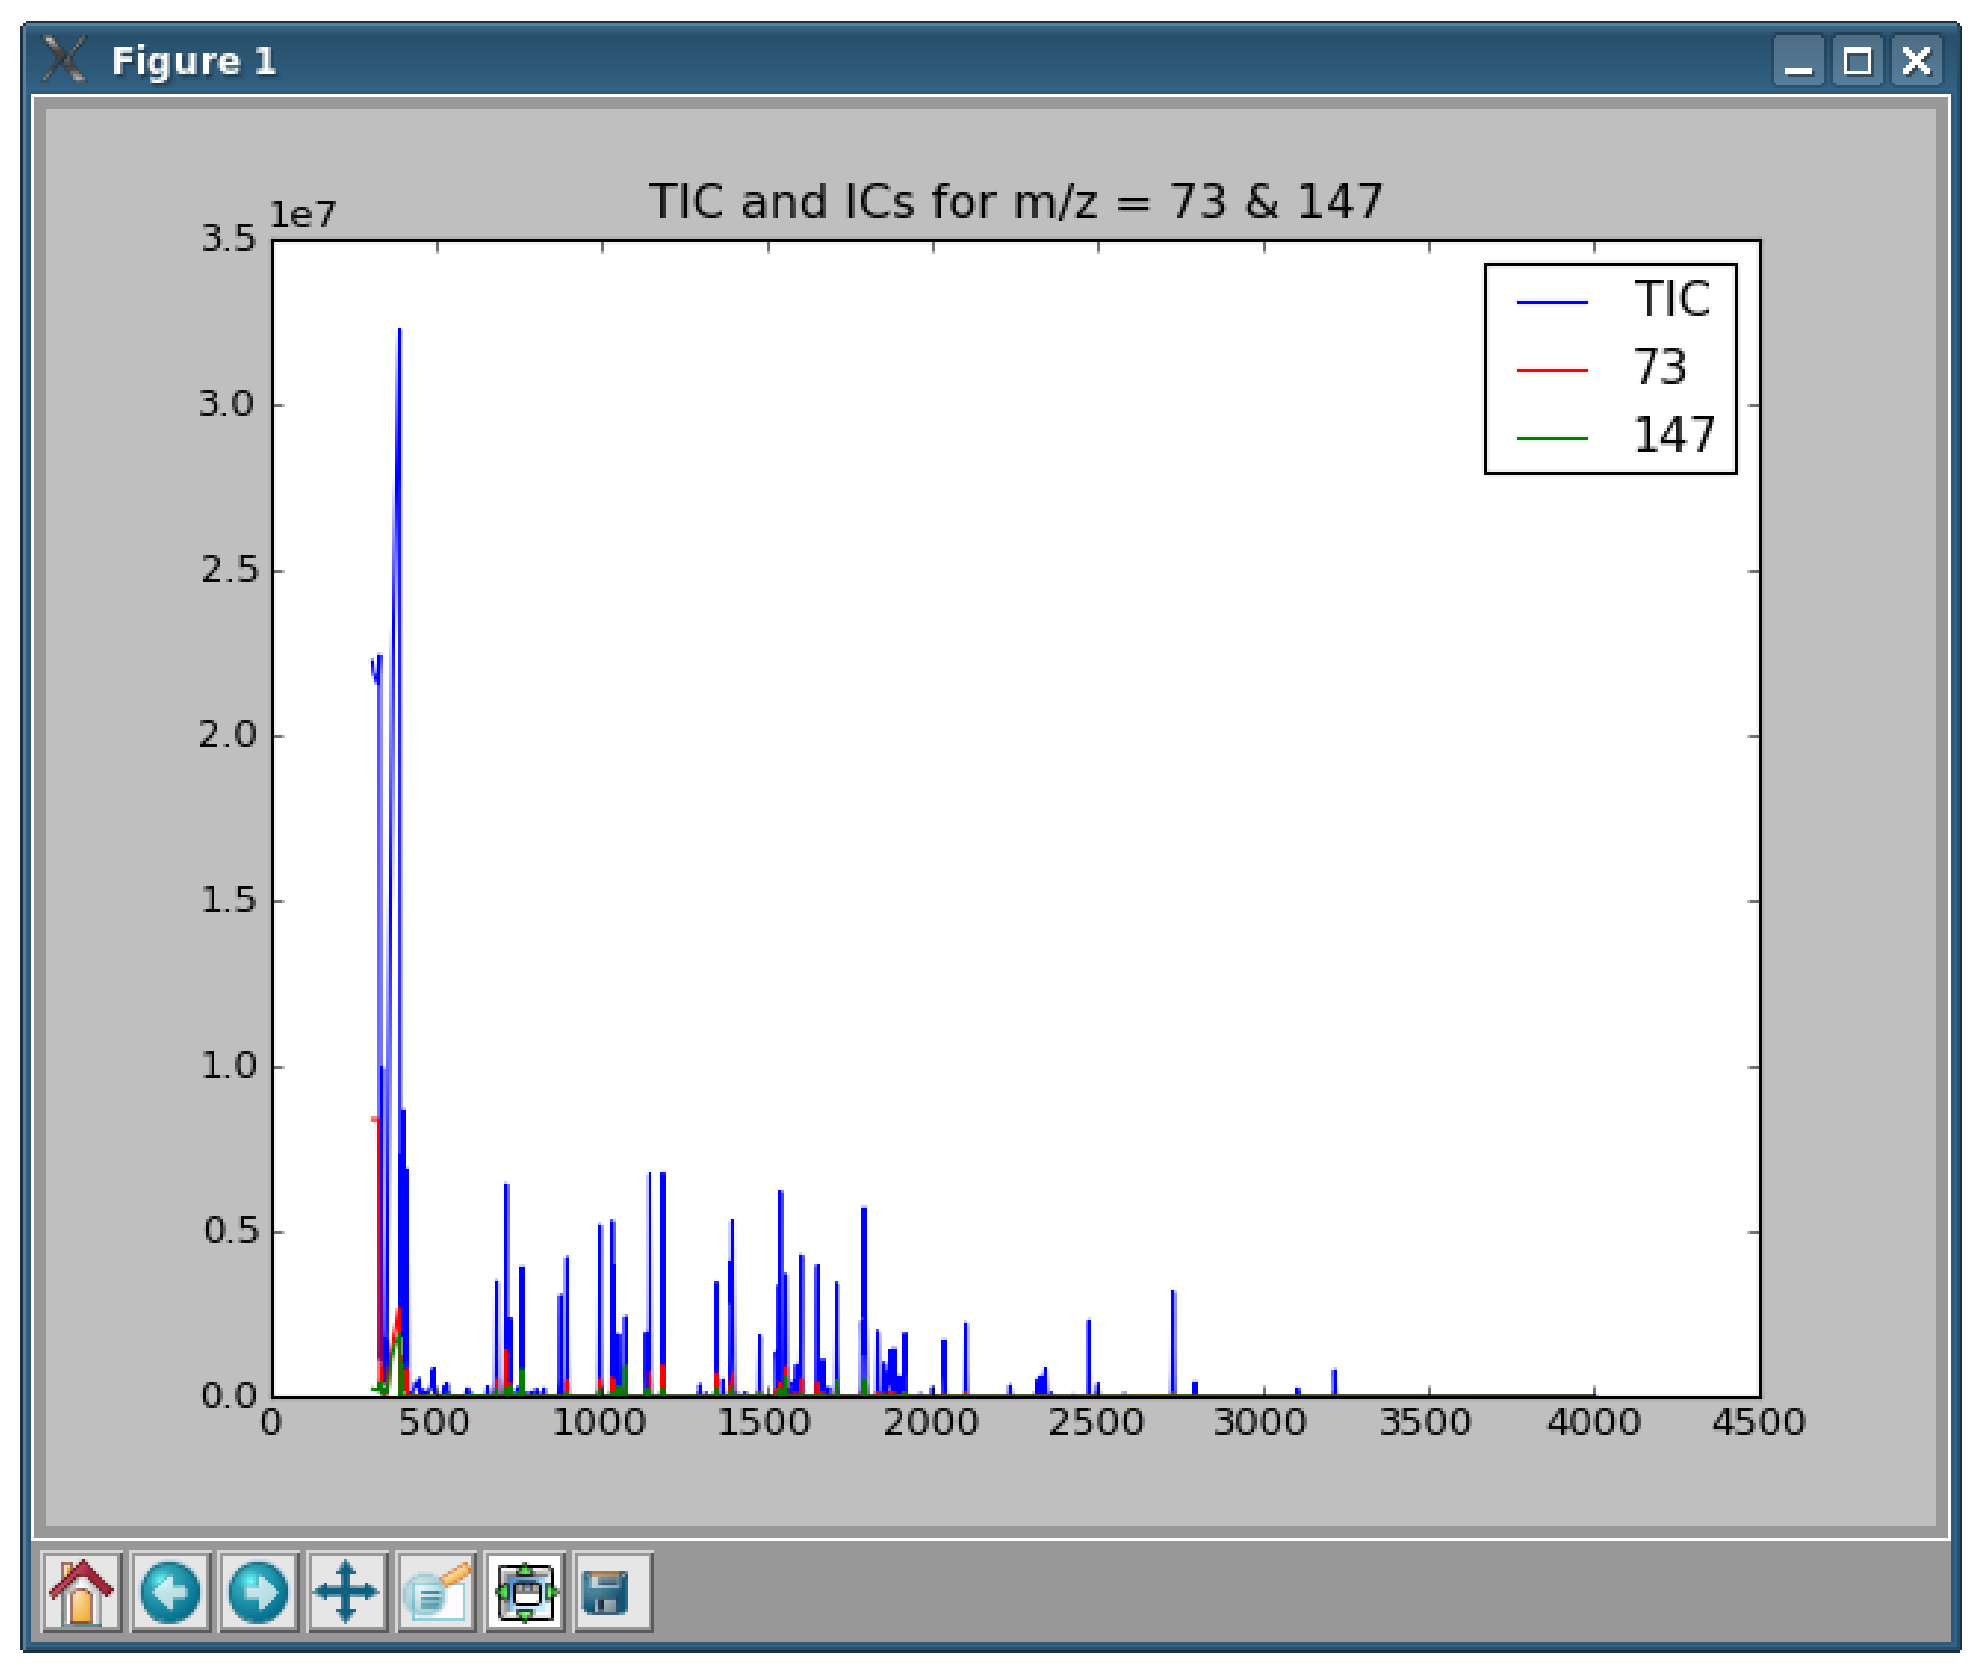
\includegraphics[scale=0.33]{graphics/chapter07/test-70b.eps}
\end{center}


\section{Displaying detected peaks on the TIC plot}

\noindent
[ {\em This example is in pyms-test/71} ]

The Display class is a more powerful implementation of plotting which 
allows plotting of detected peaks and user interaction with the plot figure.



In order to plot a list of peaks, the list must first be populated.
The script {\tt proc\_save\_peaks.py} produces such a peak list. For more information
on detecting peaks see section \ref{sec:PeakDetection}. The function 
{\tt store\_peaks()} in {\tt proc\_save\_peaks.py} stores the peaks, while
{\tt load\_peaks()} in {\tt proc.py} loads them for the Display class to use.

When using the Display Class, a series of plots is added to the figure
one at a time before the final plot is displayed.

To begin, an instance of the Display class is created:

\begin{verbatim}
>>>display = Display()
\end{verbatim}

Next some ics and the TIC are plotted. Unlike earlier examples, the TIC is
plotted using a separate function. This function ensures that the TIC is always
plotted in blue for easy reference. The legend for each IC is supplied to the
functions, but the overall figure label is not supplied at this time.

\begin{verbatim}
>>> display.plot_ics(ics, ['73','147'])
>>> displat.plot_tic(tic, 'TIC')
\end{verbatim}

The function {\tt plot\_peaks()} then adds the PyMS detected peaks to the figure.

\begin{verbatim}
>>>display.plot_peaks(peak_list, 'Peaks')
\end{verbatim}

Finally the function {\tt do\_plotting()} is called to draw the figure with 
label and display the plot.

\begin{verbatim}
>>> display.do_plotting('TIC, ICs, and PyMS Detected Peaks')
\end{verbatim}

This should result in the following window being displayed:

\begin{center}
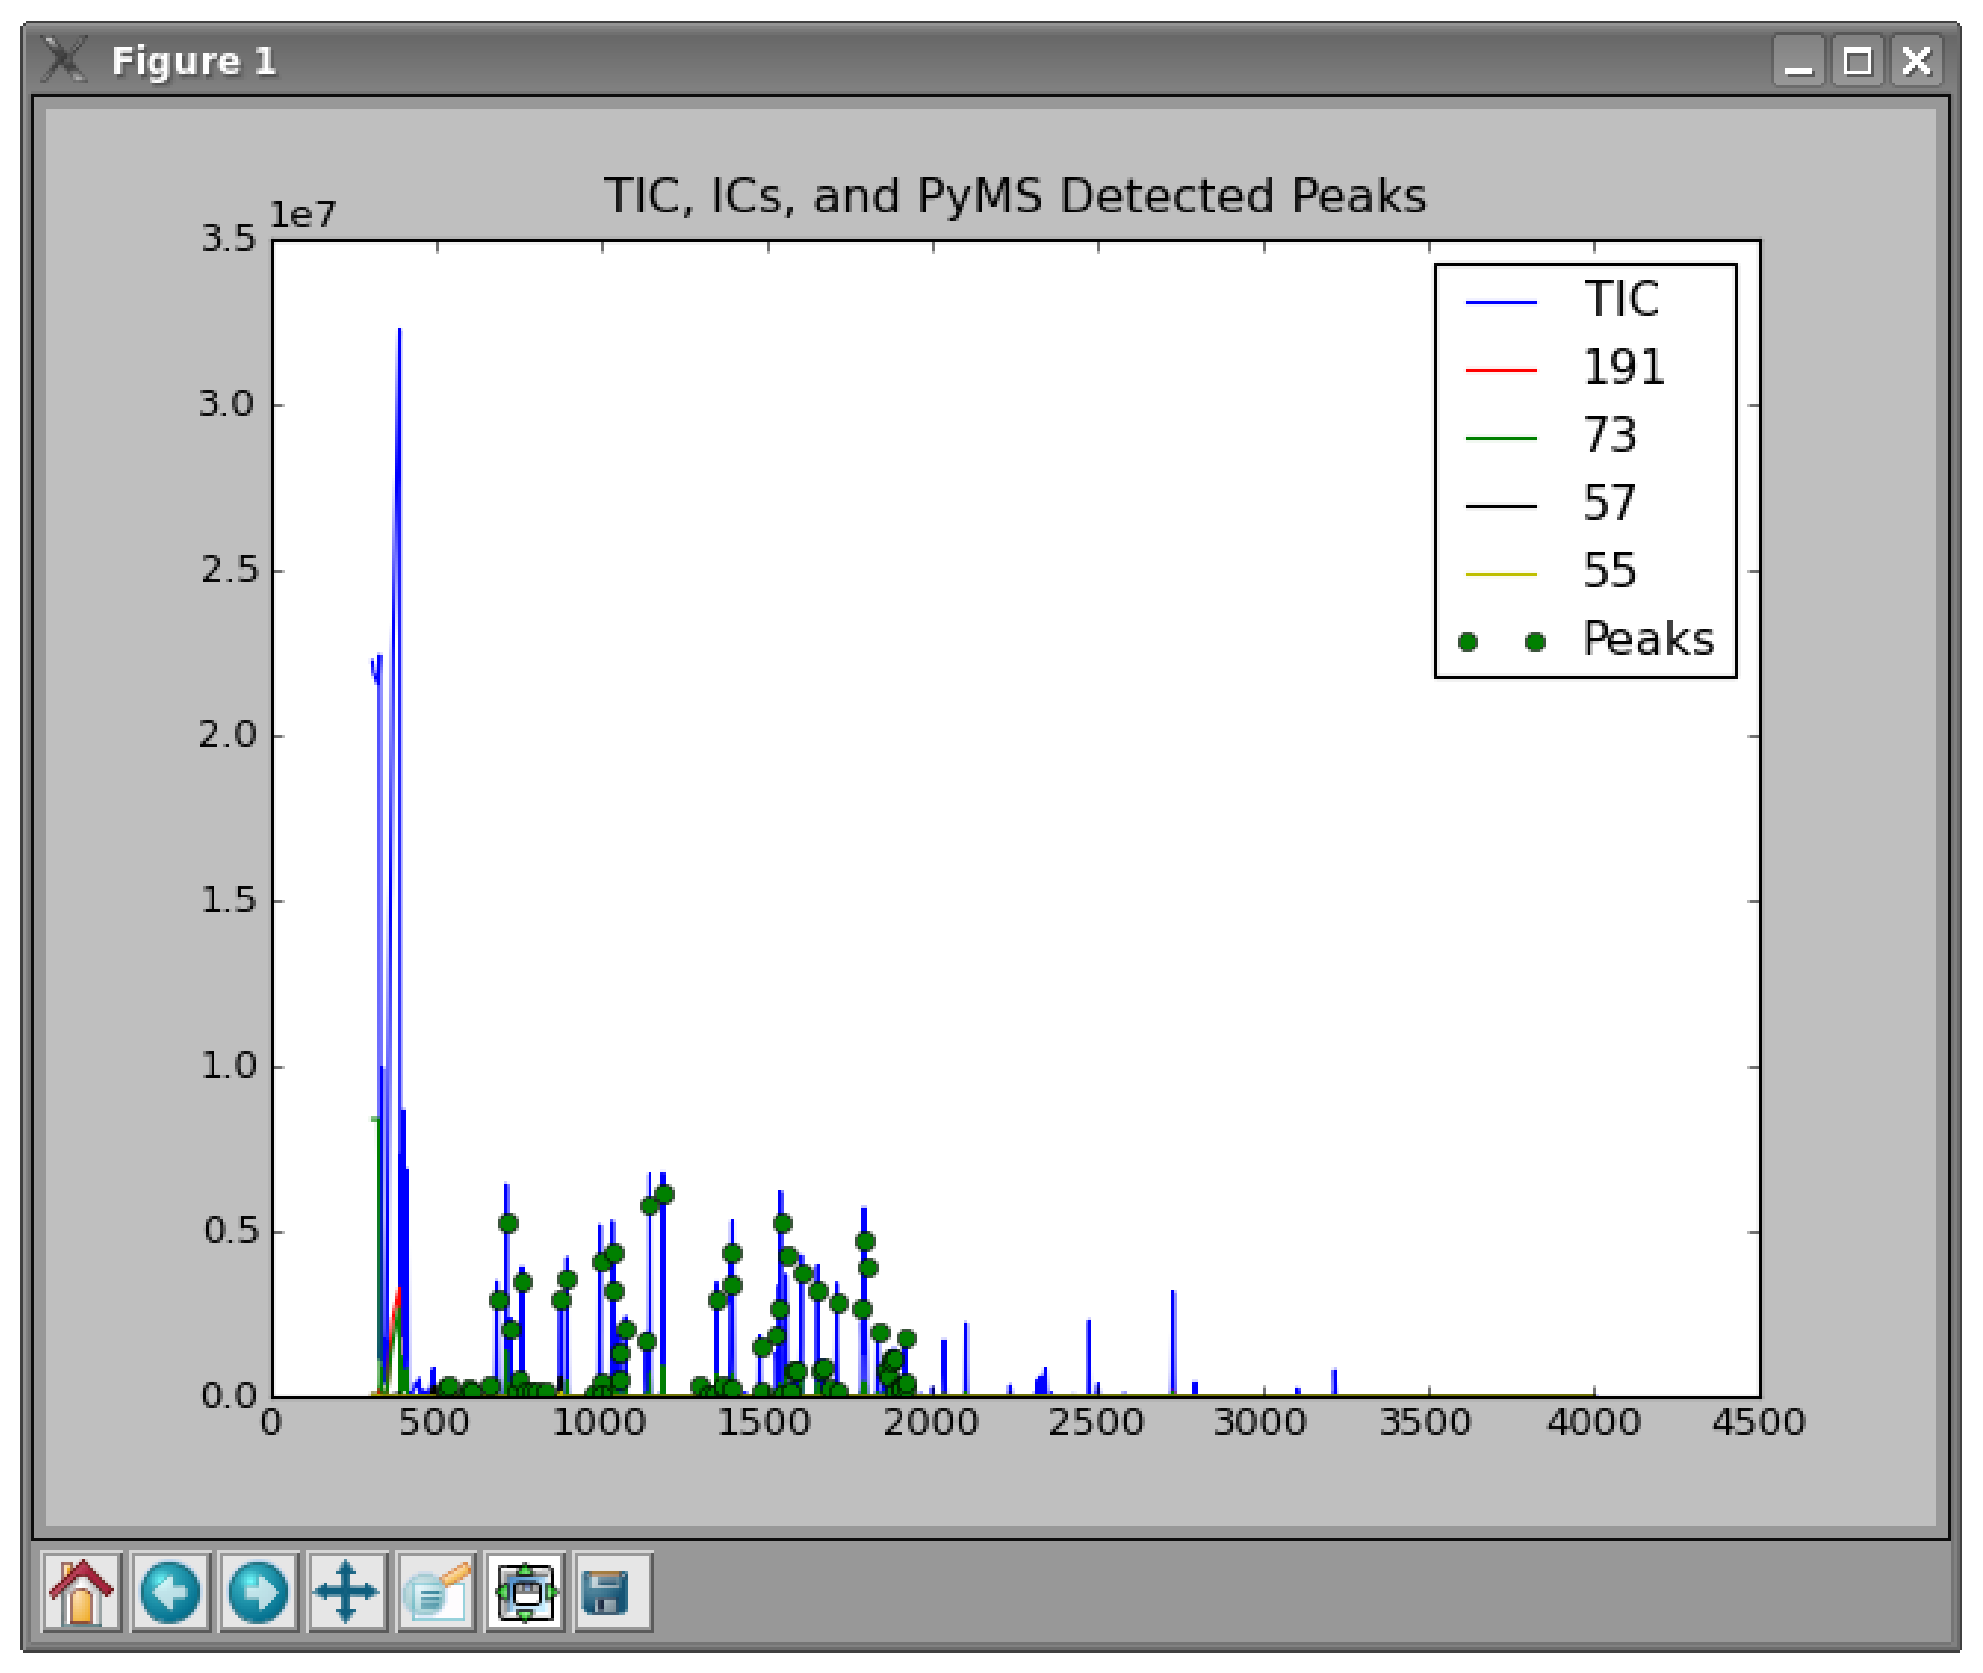
\includegraphics[scale=0.33]{graphics/chapter07/test-71-ICs.eps}
\end{center}

\subsection{User interaction with plot window}

When using the Display class, the resulting figure window can be used to
access data about the displayed peaks.

Clicking on a peak causes a list of the 5 highest intensity eluting ions at that
peak to be written to the screen in order.
Clicking a mouse button over one of the 
peaks should result in output similar to the following:

\begin{verbatim}
>>> mass     intensity
>>> 273     1003678.47619
>>> 73      625396.428571
>>> 147     526953.333333
>>> 363     255903.714286
>>> 347     241031.333333
\end{verbatim}

In addition, clicking a mouse button other than the left button on a peak displays the 
mass spectrum at the peak in a new window:

\begin{center}
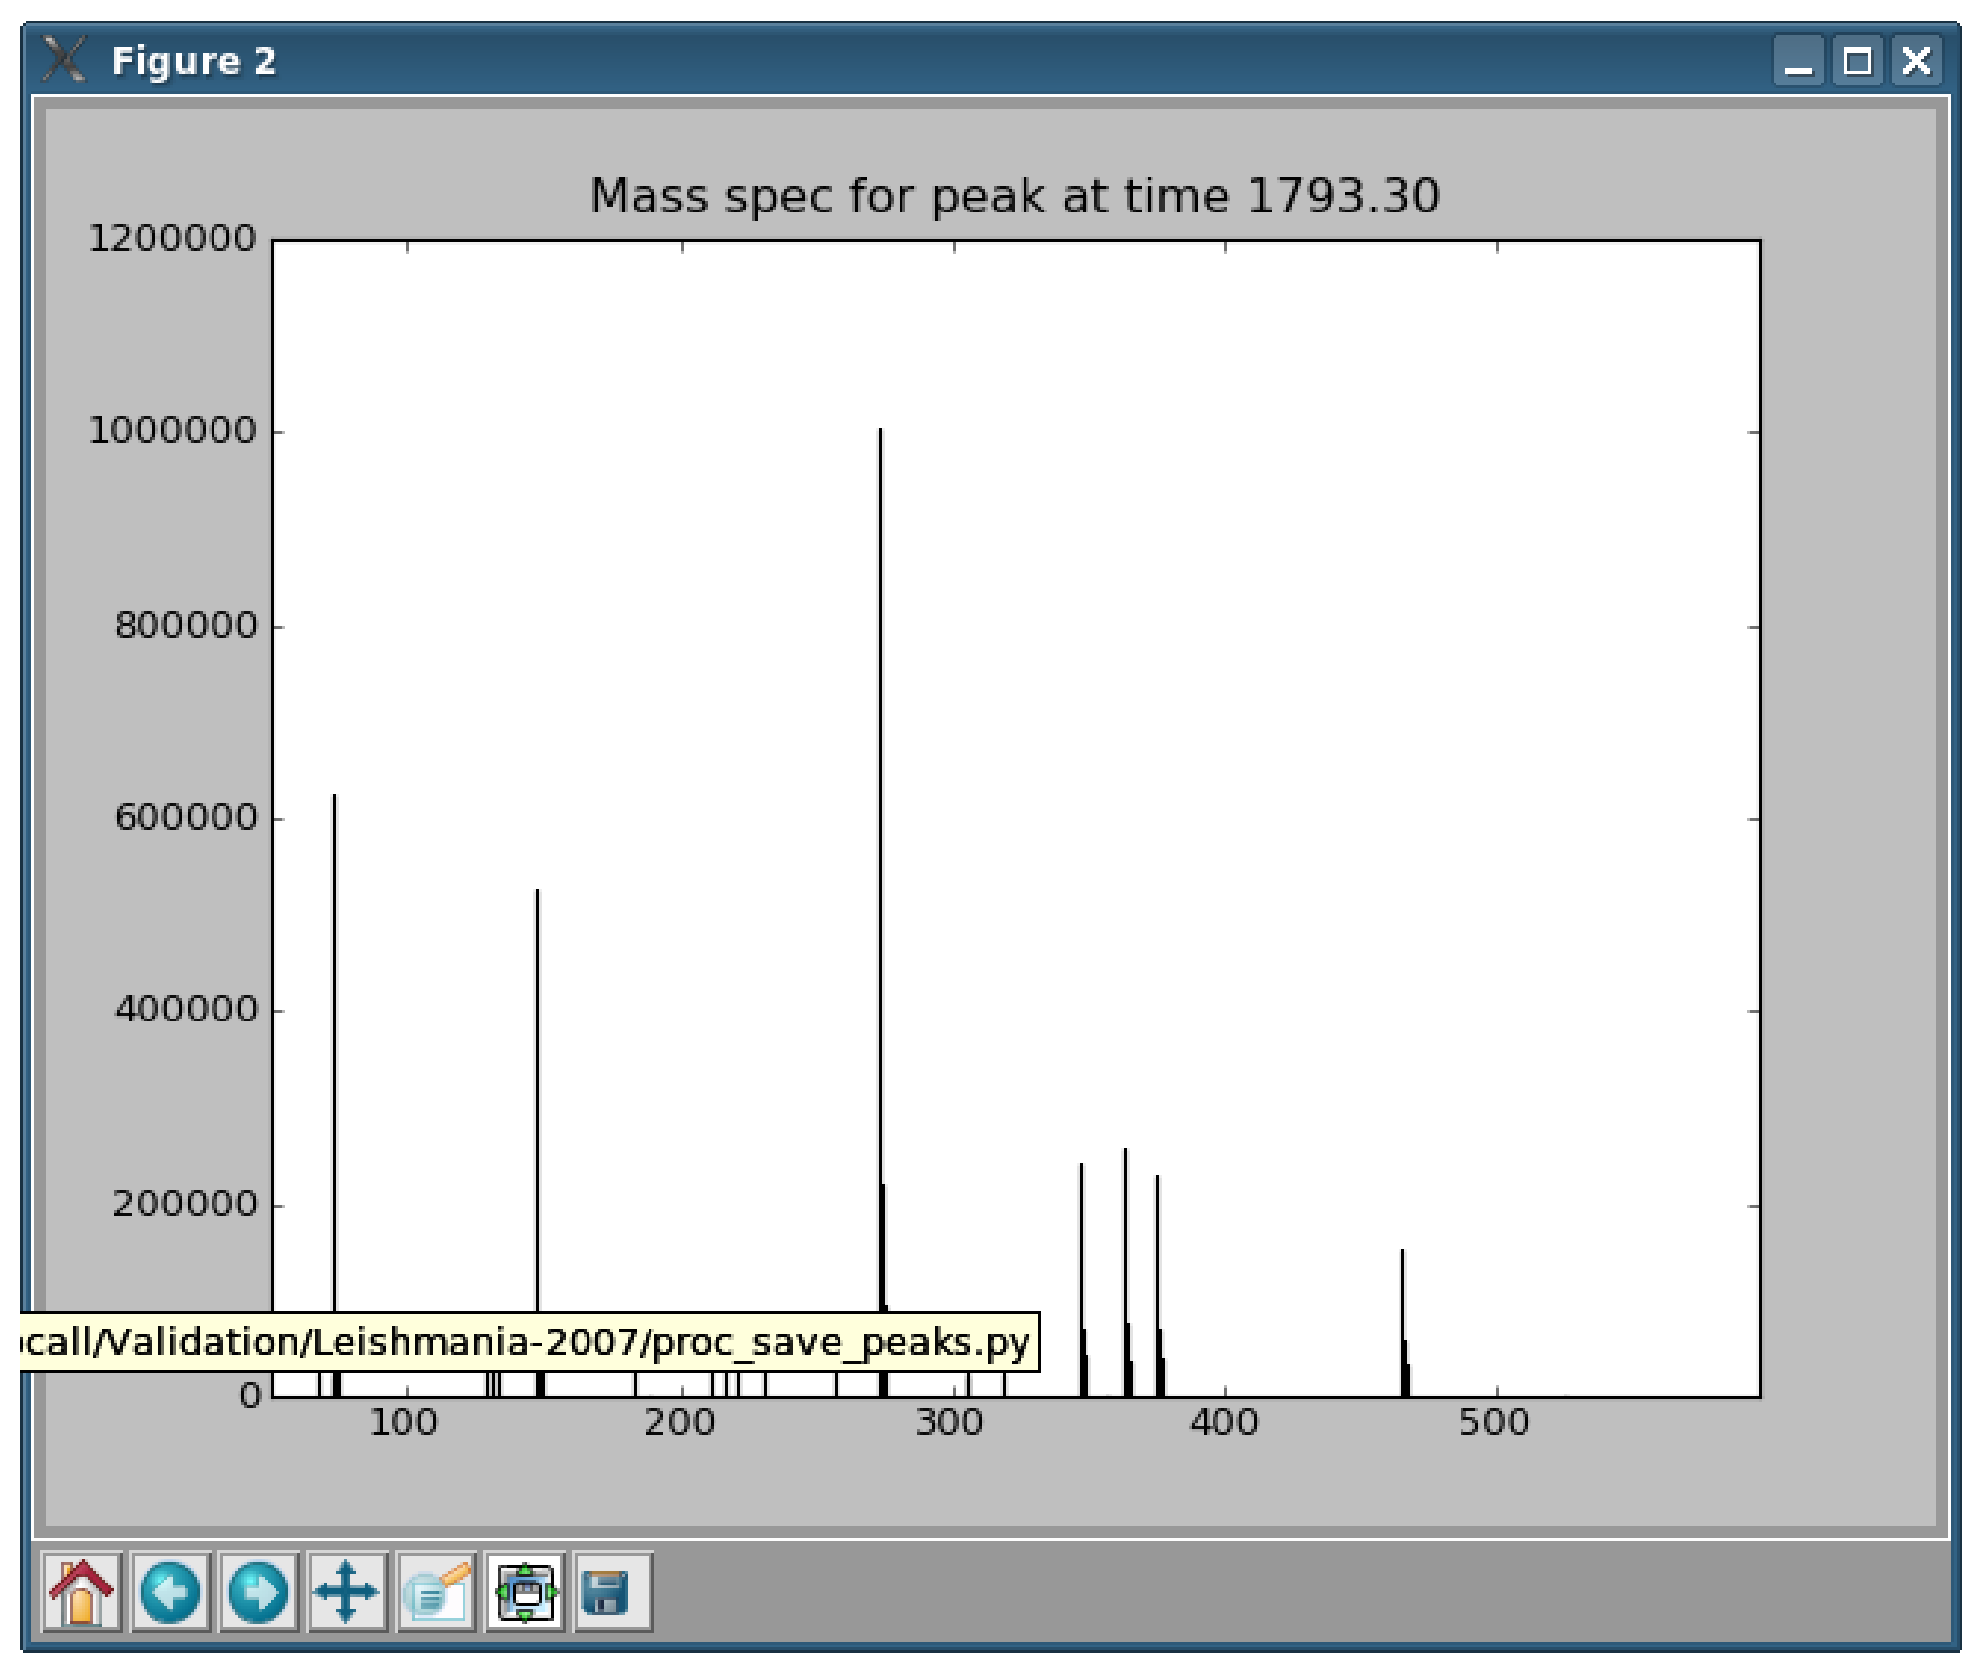
\includegraphics[scale=0.33]{graphics/chapter07/test-71-spec.eps}
\end{center}

Clicking on other peaks will display further mass spectrums for those peaks in new windows.